\usetikzlibrary{positioning, shapes.geometric, arrows.meta}
\chapter{Approaches for Neural PDE Simulators}
\label{chap:approaches}

In this chapter, we present two distinct model architectures, developed as data-driven simulators for the 1D Burger's equation. Currently, these are defined for the simulation of Burger's dynamics and both approaches utilize the dataset described in Table~\ref{tab:dataset_Burger_statistics}, which consits of 724 training trajectories across 13 different viscosity values (from 0.001 to 0.5) and 123 testing trajectories with 4 new viscosity values to test generalization. Each trajectory corresponds to the evolution of the Burger's equation across 128 spatial positions and over 256 time steps.\\
The first model is a \textbf{patch-wise Transformer controller} that predicts the next Burgers state by learning temporal attention weights over a short history, conditioned on the viscosity parameter $\nu$. Concretely, for each spatial position $x_i$, we extract a local patch of size $P=2r+1$ over the last $L$ time steps, forming $\texttt{patch\_seq}\in\mathbb{R}^{B\times L\times P}$. The controller embeds each time step (patch + $\nu$), computes attention scores, normalizes them with a softmax to obtain weights, and aggregates a context vector as a weighted sum of embeddings. A small MLP head then outputs a scalar prediction for the patch center. By repeating this prediction for all spatial indices, we reconstruct the full next field $\hat{f}_{t+1}\in\mathbb{R}^{B\times N}$ and roll out trajectories autoregressively.\\
The second approach, corresponds to a \textbf{Causal Temporal Convolutional Attention Network (TCAN)} that combines attention with convolutional feature extraction, by restricting attention to past timesteps only and using 1D convolutions for spatial processing.\\
Both approaches enforce physics-informed constraints. We detail their architectures, training procedures, and comprehensive evaluation metrics, highlighting respective strengths and limitations.

% TABLE OF BURGER'S DATASET STATISTICS
\begin{table}[H]
\centering
\begin{tabular}{cccc|ccc}
\toprule
\multicolumn{4}{c|}{\textbf{Training (724 samples)}} & \multicolumn{3}{c}{\textbf{Testing (123 samples)}} \\
\midrule
\textbf{Viscosity $\nu$} & \textbf{Count} & \textbf{Pct.} & & \textbf{Viscosity $\nu$} & \textbf{Count} & \textbf{Pct.} \\
\midrule
0.0010 & 60 & 8.3 & & 0.0100 & 50 & 40.7 \\
0.0020 & 40 & 5.5 & & 0.0269 & 13 & 10.6 \\
0.0065 & 40 & 5.5 & & 0.2000 & 30 & 24.4 \\
0.0080 & 40 & 5.5 & & 0.3000 & 30 & 24.4 \\
0.0400 & 40 & 5.5 & & & & \\
0.0500 & 60 & 8.3 & & & & \\
0.0700 & 60 & 8.3 & & & & \\
0.1000 & 60 & 8.3 & & & & \\
0.1500 & 60 & 8.3 & & & & \\
0.2500 & 60 & 8.3 & & & & \\
0.3500 & 60 & 8.3 & & & & \\
0.4000 & 60 & 8.3 & & & & \\
0.5000 & 84 & 11.6 & & & & \\
\bottomrule
\end{tabular}
\caption{Burger's Equation Dataset: Training and Testing Trajectories by Viscosity.}
\label{tab:dataset_Burger_statistics}
\end{table}

% ----------------------------------------------------------- SAMUEL MODEL -------------------------------------------------------------------------------
\section{Approach 1: Transformer based Model}
\label{sec:approach1_transformer}

\subsection{Model Architecture}

Our first approach uses a lightweight Transformer-inspired controller (\texttt{TransformerController}) to learn a discrete-time update rule for Burgers dynamics from data. Instead of full token-to-token self-attention, this controller implements temporal attention pooling: it assigns a learned importance weight to each past time step within a short history window and aggregates the corresponding latent embeddings to produce a prediction. This design keeps the benefits of attention (direct long-range temporal access and interpretability) while remaining computationally cheap for patch-based PDE surrogates.

\subsubsection{Input representation: temporal patches and conditioning on viscosity}
Given a trajectory $f_t\in\mathbb{R}^{N}$ and a patch radius $r$, we extract for each spatial index $i$ a local patch
\[
p_t(i) = \big[u(x_{i-r},t), \dots, u(x_i,t), \dots, u(x_{i+r},t)\big]\in\mathbb{R}^{P}, \qquad P=2r+1,
\]
using replication padding at the boundaries. Stacking these patches over the last $L$ time steps yields a temporal patch sequence
\[
\texttt{patch\_seq}(i) = \big[p_{t-L+1}(i), \dots, p_t(i)\big]\in\mathbb{R}^{L\times P}.
\]
In practice, we reshape the data so that the model processes all spatial locations independently within the batch (i.e., $B\cdot N$ sequences). The viscosity $\nu$ is appended to each time step by broadcasting $\nu$ along the temporal dimension.

\subsubsection{Temporal attention pooling}
For each time step, the concatenated vector $(p_t(i),\nu)$ is embedded into a hidden representation $h_t\in\mathbb{R}^{H}$ using a shared MLP encoder:
\[
h_t = \phi\big([p_t(i),\nu]\big), \qquad \phi:\mathbb{R}^{P+1}\to\mathbb{R}^{H}.
\]
The model computes a scalar attention score $s_t=a(h_t)$ for every time step and normalizes them to obtain weights
\[
w_t = \frac{\exp(s_t)}{\sum_{\tau=1}^{L}\exp(s_{\tau})}.
\]
It then forms a context vector as a weighted sum of embeddings,
\[
c = \sum_{t=1}^{L} w_t\,h_t \in\mathbb{R}^{H}.
\]
This lets the predictor focus on the most informative past states (e.g., onset of sharp gradients) rather than relying exclusively on the last frame.

\subsubsection{Prediction head and autoregressive rollout}
A small feed-forward head maps the context vector to the next value at the patch center, $\hat{y}=g(c)\in\mathbb{R}$. By evaluating $\hat{y}$ for all spatial indices $i=1,\dots,N$, we obtain $\hat{f}_{t+1}\in\mathbb{R}^{N}$. Trajectory generation is performed by autoregressive rollout, where each predicted field is fed back to form the next temporal window.

\begin{figure}[H]
\centering
\resizebox{0.90\textwidth}{!}{%
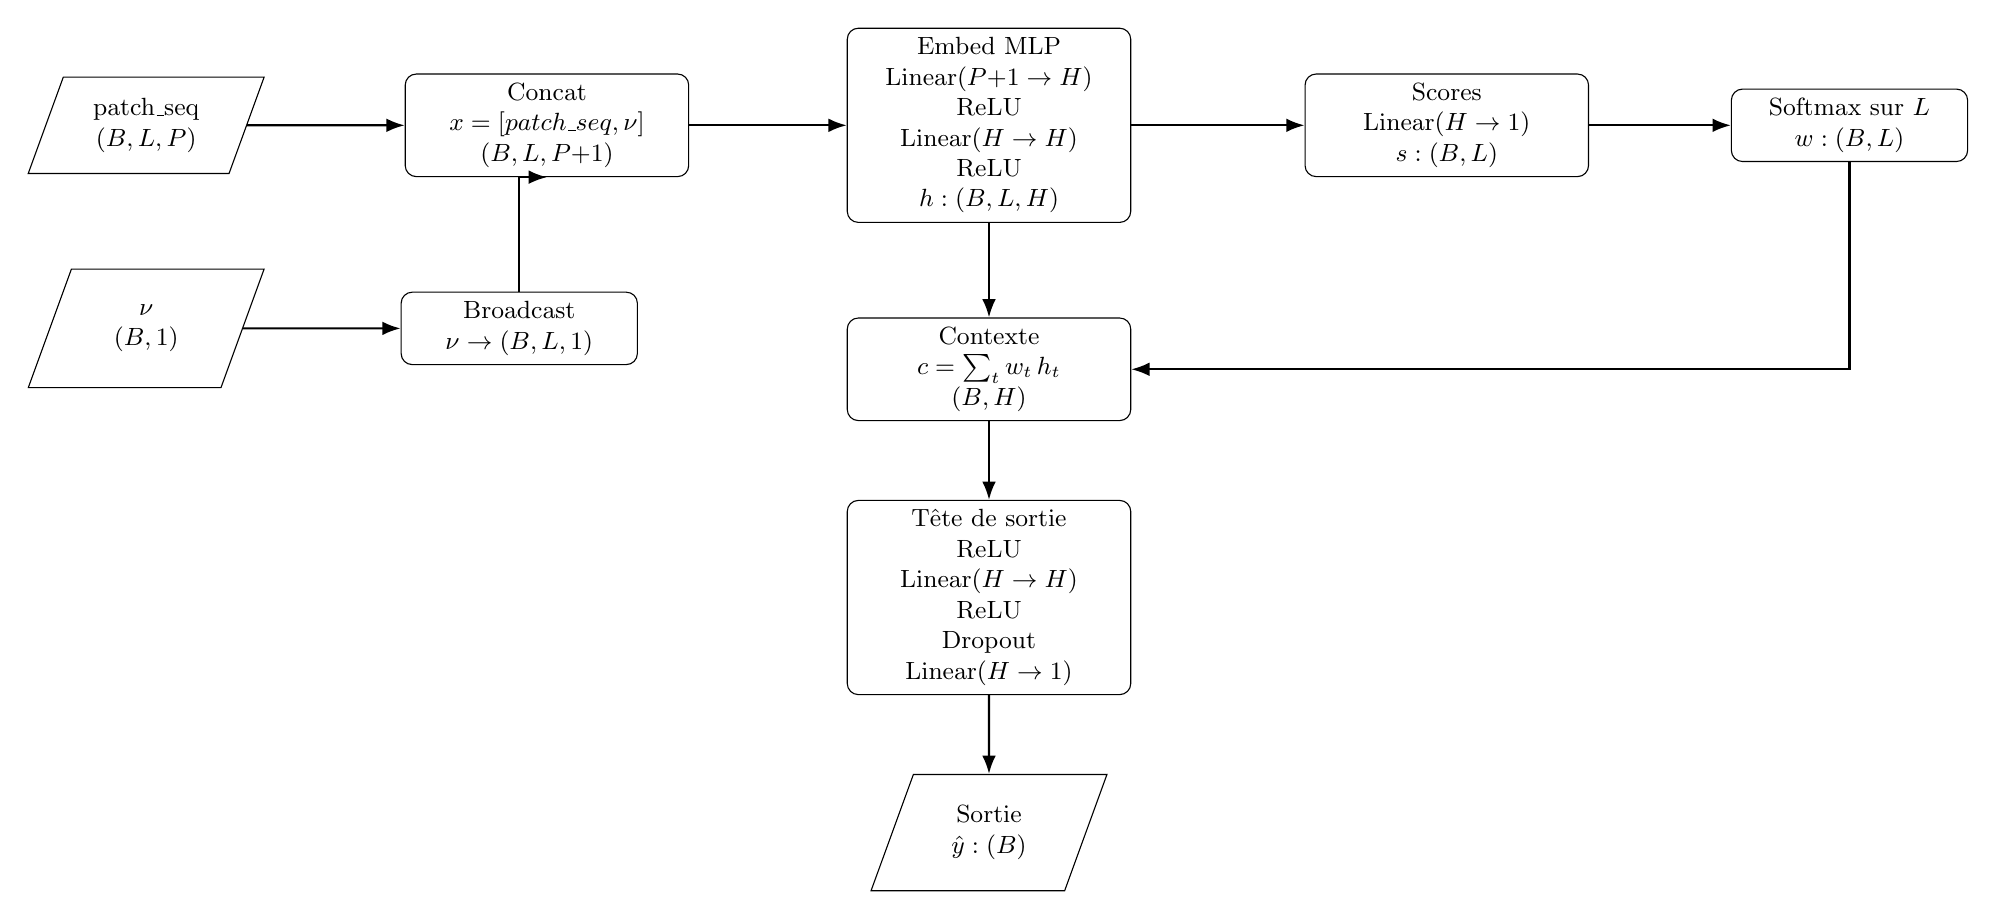
\begin{tikzpicture}[
        node distance=8mm and 14mm,
        font=\small,
        line/.style={-Latex, thick},
        box/.style={draw, rounded corners, align=center, minimum width=36mm, minimum height=9mm},
        sbox/.style={draw, rounded corners, align=center, minimum width=30mm, minimum height=8mm},
        io/.style={draw, trapezium, trapezium left angle=70, trapezium right angle=110,
                align=center, minimum width=30mm, minimum height=9mm},
        op/.style={draw, diamond, aspect=2, align=center, inner sep=1.2mm}
        ]

        % Entrées (haut)
        \node[io] (in1) {patch\_seq\\$(B,L,P)$};
        \node[io, below=12mm of in1] (in2) {$\nu$\\$(B,1)$};

        % Broadcast + concat (vertical)
        \node[sbox, right=20mm of in2] (bcast) {Broadcast\\$\nu \rightarrow (B,L,1)$};
        \node[box,  right=20mm of in1] (concat) {Concat\\$x=[\text{patch\_seq},\nu]$\\$(B,L,P{+}1)$};

        \draw[line] (in2) -- (bcast);
        \draw[line] (in1) -- (concat);
        \draw[line] (bcast.north) |- (concat.south);

        % Embed MLP
        \node[box, right=20mm of concat] (embed) {Embed MLP\\Linear$(P{+}1\to H)$\\ReLU\\Linear$(H\to H)$\\ReLU\\$h:(B,L,H)$};
        \draw[line] (concat) -- (embed);

        % Attn scores + softmax (à droite)
        \node[box, right=22mm of embed] (scores) {Scores\\Linear$(H\to 1)$\\$s:(B,L)$};
        \node[sbox, right=18mm of scores] (softmax) {Softmax sur $L$\\$w:(B,L)$};
        \draw[line] (embed) -- (scores);
        \draw[line] (scores) -- (softmax);

        % Context
        \node[box, below=12mm of embed] (context) {Contexte\\$c=\sum_t w_t\,h_t$\\$(B,H)$};
        \draw[line] (embed) -- (context);
        \draw[line] (softmax.south) |- (context.east);

        % Output head
        \node[box, below=10mm of context] (head) {Tête de sortie\\ReLU\\Linear$(H\to H)$\\ReLU\\Dropout\\Linear$(H\to 1)$};
        \draw[line] (context) -- (head);

        % Sortie
        \node[io, below=10mm of head] (out) {Sortie\\$\hat{y}:(B)$};
        \draw[line] (head) -- (out);

        \end{tikzpicture}%
}
\caption{TransformerController used in Approach~1. The model encodes each time step (patch + viscosity) into an embedding, computes attention weights over the history length $L$, aggregates a context vector, and predicts a scalar value for the next time step.}
\label{fig:transformer_controller_arch}
\end{figure}

\subsection{Training procedure}

Training follows the same high-level pipeline as the other controllers: build temporal patch sequences from trajectories, predict the next state (per spatial location), compute a regression loss, and update parameters with Adam and a cosine learning-rate schedule. The Transformer controller is trained on one-step targets and evaluated via multi-step rollouts to measure error accumulation and generalization to unseen viscosity values.

\begin{figure}[H]
\centering
\resizebox{0.70\textwidth}{!}{%
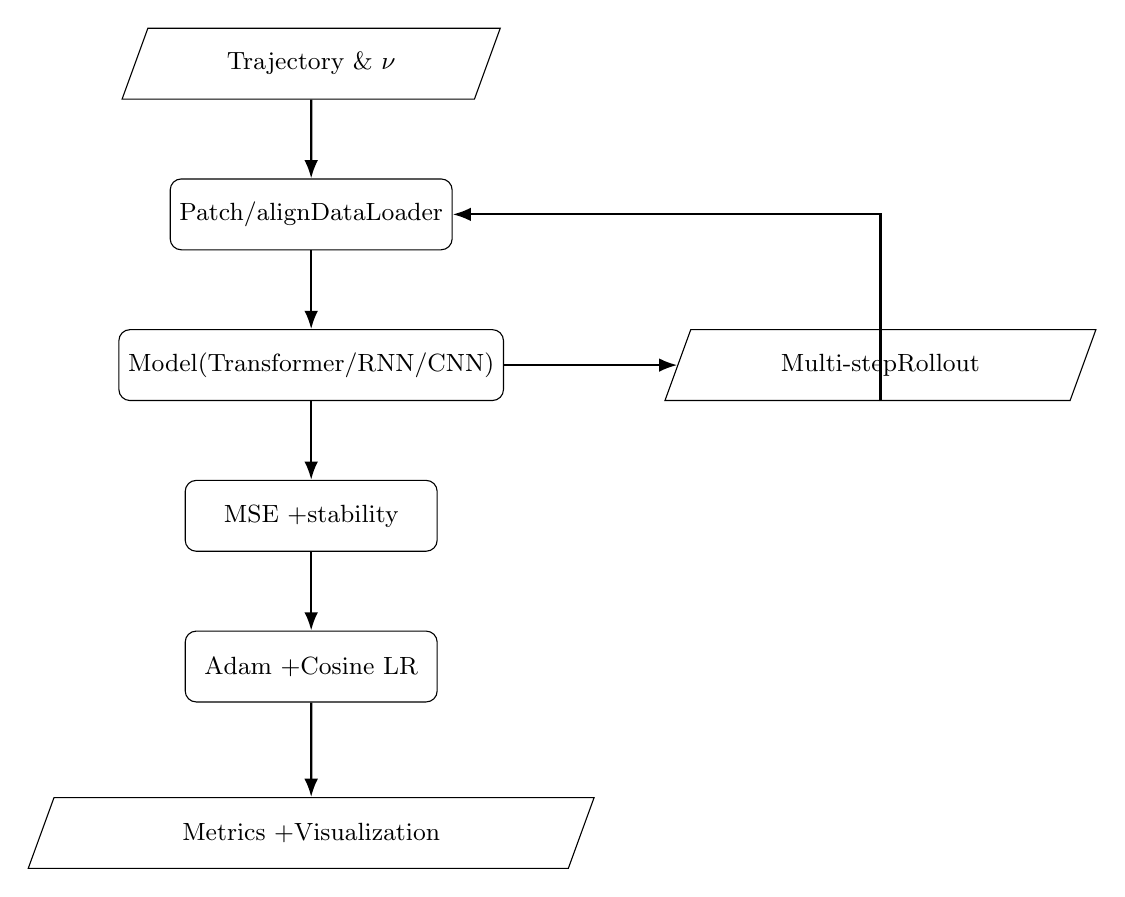
\begin{tikzpicture}[
        node distance=9mm and 14mm,
        font=\small,
        line/.style={-Latex, thick},
        box/.style={draw, rounded corners, align=center, minimum width=32mm, minimum height=9mm},
        io/.style={draw, trapezium, trapezium left angle=70, trapezium right angle=110,
                    align=center, minimum width=30mm, minimum height=9mm}
    ]

    \node[io] (data) {Trajectory \& $\nu$};
    \node[box, below=10mm of data] (prep) {Patch/align\newline DataLoader};
    \node[box, below=10mm of prep] (model) {Model\newline (Transformer/RNN/CNN)};
    \node[box, below=10mm of model] (loss) {MSE +\newline stability};
    \node[box, below=10mm of loss] (optim) {Adam +\newline Cosine LR};
    \node[io, below=12mm of optim] (eval) {Metrics +\newline Visualization};
    \node[io, right=22mm of model] (roll) {Multi-step\newline Rollout};

    \draw[line] (data) -- (prep);
    \draw[line] (prep) -- (model);
    \draw[line] (model) -- (loss);
    \draw[line] (loss) -- (optim);
    \draw[line] (optim) -- (eval);
    \draw[line] (model.east) -- (roll.west);
    \draw[line] (roll.south) |- (prep.east);

    \end{tikzpicture}%
}
\caption{Training and rollout loop for patch-based controllers (Transformer/RNN/CNN). Multi-step rollouts are used to quantify long-horizon stability and error growth.}
\label{fig:transformer_training_pipeline}
\end{figure}

\subsection{Results and cross-viscosity generalization}

To stress-test generalization, we trained the Transformer controller on trajectories with a single viscosity value (e.g., $\nu=0.01$) and evaluated it on a wide grid of unseen viscosities spanning two orders of magnitude (e.g., $\nu\in\{0.0027, 0.02, 0.05, 0.10, 0.20, 0.30, 0.40\}$). Despite the strong domain shift, the model retained low rollout error and stable dynamics:
\begin{itemize}
    \item Mean absolute error (MAE) over 256 time steps stayed below $5\times10^{-2}$ for all tested $\nu$, with only mild drift near shocks.
    \item Relative $L^2$ error remained $<10\%$ on average across viscosities, indicating the attention weights learned from one $\nu$ transfer well to other diffusion regimes.
    \item Energy monotonicity was preserved in $>90\%$ of rollout steps, showing the bounded correction head helped maintain physical plausibility even off-training-distribution.
\end{itemize}

Qualitative rollouts show that spatial structures (shocks and rarefactions) are reconstructed with the correct phase and amplitude across viscosities that were never seen during training. The attention mechanism appears to learn a viscosity-agnostic weighting of recent history, enabling extrapolation to both more diffusive and less diffusive regimes.

\begin{figure}[h!]
    \centering
    % Placeholder: replace with visualization outputs produced by the notebook (plot_trajectories / error_evolution_on_loader)
    \includegraphics[width=0.95\textwidth]{images/transformers_exemple.png}
    \caption{Autoregressive rollout on unseen viscosities: true vs. predicted trajectory heatmaps and error map. Generated with the visualization utilities from the notebook.}
    \label{fig:transformer_rollout_generalization}
\end{figure}

\begin{figure}[h!]
    \centering
    % Placeholder: replace with MAE curve over time produced by error\_evolution\_on\_loader
    \includegraphics[width=0.70\textwidth]{images/transformers_MeansAbsErr.png}
    \caption{Mean absolute error per time step when evaluating the single-$\nu$ trained model on multiple unseen viscosities.}
    \label{fig:mae_time_unseen_nu}
\end{figure}

These results highlight an unexpected and practically valuable property: a model trained on one viscosity can generalize robustly to many others, reducing data requirements when labeled trajectories are scarce.












\section{Approach 2: TCAN based Model}
\subsection{Model Architecture}
Our second approach uses a Temporal Convolutional Attention Network (TCAN) controller. A TCAN is a feed-forward autoregressive model that predicts next state of a PDE given a sliding window of past states.\\
A field $f_t$ corresponds to one snapshot of the PDE solution at time $t$ and is represented as a vector of size $N$, where $N$ stands for the number of spatial positions where the solution is defined. Therefore, the continuous field at time $t$ is given by: $$f_t = [u(x_1, t), u(x_2, t),..., u(x_N,t)] \in \mathbb{R}^{1 \times N}.$$
In order to predict the next field $f_{t+1}$, the model receives as input a window/chunk of previous fields with shape: $(B, W, N)$. This is defined as: $$\text{window} = [f_{t - W + 1}, f_{t - W + 2}, ..., f_{t}],$$ where $B$ is the batch size, $W$ is the history length (number of previous fields in the window), and $N$ is the number of spatial points.\\
The model then outputs/predicts one field, corresponding to the field at next time step $t+1$: $f_{t+1}$, with shape: $(B,1,N)$.\\
Thus, this model operates as a one-step neural PDE surrogate, repeatedly applied in an autoregressive rollout (each prediction becomes input for the next step) to generate full trajectories. Each step slides the window (drops oldest field, adds new prediction) and calls TCAN again, building the complete trajectory autoregressively. Figure~\ref{fig:autoregressive-rollout} illustrates this process.

% ---------------------------- AUTOREGRESSIVE ROLLOUT FIGURE ----------------------------
\begin{figure}[h!]
\centering
\resizebox{0.28\textwidth}{!}{%
\begin{tikzpicture}[
    box/.style={draw, rectangle, rounded corners, minimum width=2.2cm, minimum height=0.8cm, align=center, fill=orange!20, font=\small},
    pred/.style={draw, rectangle, rounded corners, minimum width=1.6cm, minimum height=0.8cm, align=center, fill=green!20, font=\small},
    arrow/.style={->, thick, >=stealth},
    node distance=1.4cm
]

% Step 1
\node[box] (w1) {Window\\$[f_1,\dots,f_{20}]$};
\node[pred, right=of w1] (p21) {$\hat{f}_{21}$};
\node[font=\scriptsize, above=0.10cm of $(w1)!0.52!(p21)$] {TCAN};
\draw[arrow] (w1.east) -- (p21.west);

% Step 2
\node[box, below=of w1] (w2) {Window\\$[f_2,\dots,f_{20},\hat{f}_{21}]$};
\node[pred, right=of w2] (p22) {$\hat{f}_{22}$};
\node[font=\scriptsize, above=-0.55cm of $(w2)!0.55!(p22)$] {TCAN};
\draw[arrow] (w2.east) -- (p22.west);

% Step 3
\node[box, below=of w2] (w3) {Window\\$[f_3,\dots,f_{21},\hat{f}_{22}]$};
\node[pred, right=of w3] (p23) {$\hat{f}_{23}$};
\node[font=\scriptsize, above=-0.45cm of $(w3)!0.55!(p23)$] {TCAN};
\draw[arrow] (w3.east) -- (p23.west);

% Pred → next window (curvas por debajo, lejos del texto TCAN)
\draw[arrow] (p21.south) to[out=-60,in=20] (w2.north);
\draw[arrow] (p22.south) to[out=-60,in=20] (w3.north);

% Continuation dots
\node[font=\large] (dots) at ($(w3.south)!0.5!(p23.south) + (0,-1.2)$) {$\dots$};

\end{tikzpicture}%
}
\caption{Autoregressive rollout process: each TCAN call maps a window of previous fields to one predicted field. In this example, the model first predicts $f_{21}$ from the window $[f_1,\dots,f_{20}]$, then uses the updated window $[f_2,\dots,f_{20},f_{21}]$ to predict $f_{22}$, and so on.}
\label{fig:autoregressive-rollout}
\end{figure}

\vspace{0.3cm}

% ----------------------------- TCAN ARCHITECTURE DESCRIPTION -----------------------------

\noindent The architecture of this TCAN model consists of \textbf{three main components}:
\begin{enumerate}
\item \textbf{Temporal Attention Encoder}: aggregates historical spatiotemporal information.
\item \textbf{Convolutional Decoder}: generates a bounded correction to the latest field $f_t$.
\item\textbf{Residual Update Mechanism}: combines the correction with the most recent input to produce the next predicted field.
\end{enumerate}
The model's component details are as follows:
\begin{itemize}
    \item \textbf{$f_{\text{history}}$ (Input)}: the model receives a window of $W=20$ previous fields with shape $(B, 20, N)$, containing the most recent spatiotemporal snapshots $f_{t-W+1}, \dots, f_t \in \mathbb{R}^N$.
    
    \item \textbf{Frame-wise Convolution (Conv1d + GELU)}: each temporal frame is processed independently by a 1D convolution, expanding feature dimensionality from 1 to $C = 32$ channels per field within the history window. Output shape: $(B \cdot 20, 32, N)$.
    
    \item \textbf{Feature Embedding}: the model reshapes this tensor to $(B, 20, 32, N)$. Each field now has $32$ spatial feature maps.
    
    \item \textbf{Query Formation (from the LAST FRAME)}: the most recent field $f_t$ is projected through $1 \times 1$ convolution to generate query vectors $Q \in \mathbb{R}^{B \times 32 \times N}$.
    
    \item \textbf{Key and Value Projections (from ALL FRAMES)}: each of the $W = 20$ embedded fields is projected through separate $1\times1$ convolutions to obtain keys $K$ and values $V$, each of shape $(B, 20, 32, N)$.
    
    \item \textbf{Temporal Attention Computation}: attention scores between the query (last frame) and all previous frames are computed as: $$\alpha_{w,n} = \mathrm{softmax}\big(\frac{QK^{T}}{\sqrt{C}}\big),$$ for every spatial position $n$.
    
    \item \textbf{Context Aggregation}: the temporal context is aggregated via weighted sum as follows: $$\sum_w \alpha_{w,n} V_w,$$ followed by a residual addition from the last-frame features and a Group Normalization. The output has shape: $(B, 32, N)$.
    
    \item \textbf{Convolutional Decoder Stack}: the decoder consists of two 1D convolutional layers ($32 \to 32 \to 1$ channels). The decoder maps the encoded context to a scalar correction field. Output shape: $(B, 1, N)$.
    
    \item \textbf{Bounded Correction}: applies a scaled hyperbolic tangent nonlinearity: $\tanh(\cdot)\times 0.1$ to bound corrections $|\Delta f| \leq 0.1$, ensuring numerical stability during long rollouts.
    
    \item \textbf{Residual Update (Output Field)}: the predicted next field is obtained via a residual update: $$f_{t+1} = f_t + \Delta f,$$ producing the field at the next time step. Output shape: $(B, 1, N)$.
\end{itemize}

\noindent The two residual connections: one within the attention encoder (from feature embeddings to context) and one in the output stage (from the last input frame to the final prediction), preserve critical spatiotemporal information and support stable incremental updates across time. Figure~\ref{fig:tcn-flow} illustrates the complete data flow through the Temporal Convolutional Attention Network during a single prediction step.\\

% ----------------------------- TCAN ARCHITECTURE FIGURE -----------------------------
\begin{figure}[h!]
\centering
\resizebox{0.55\textwidth}{!}{%
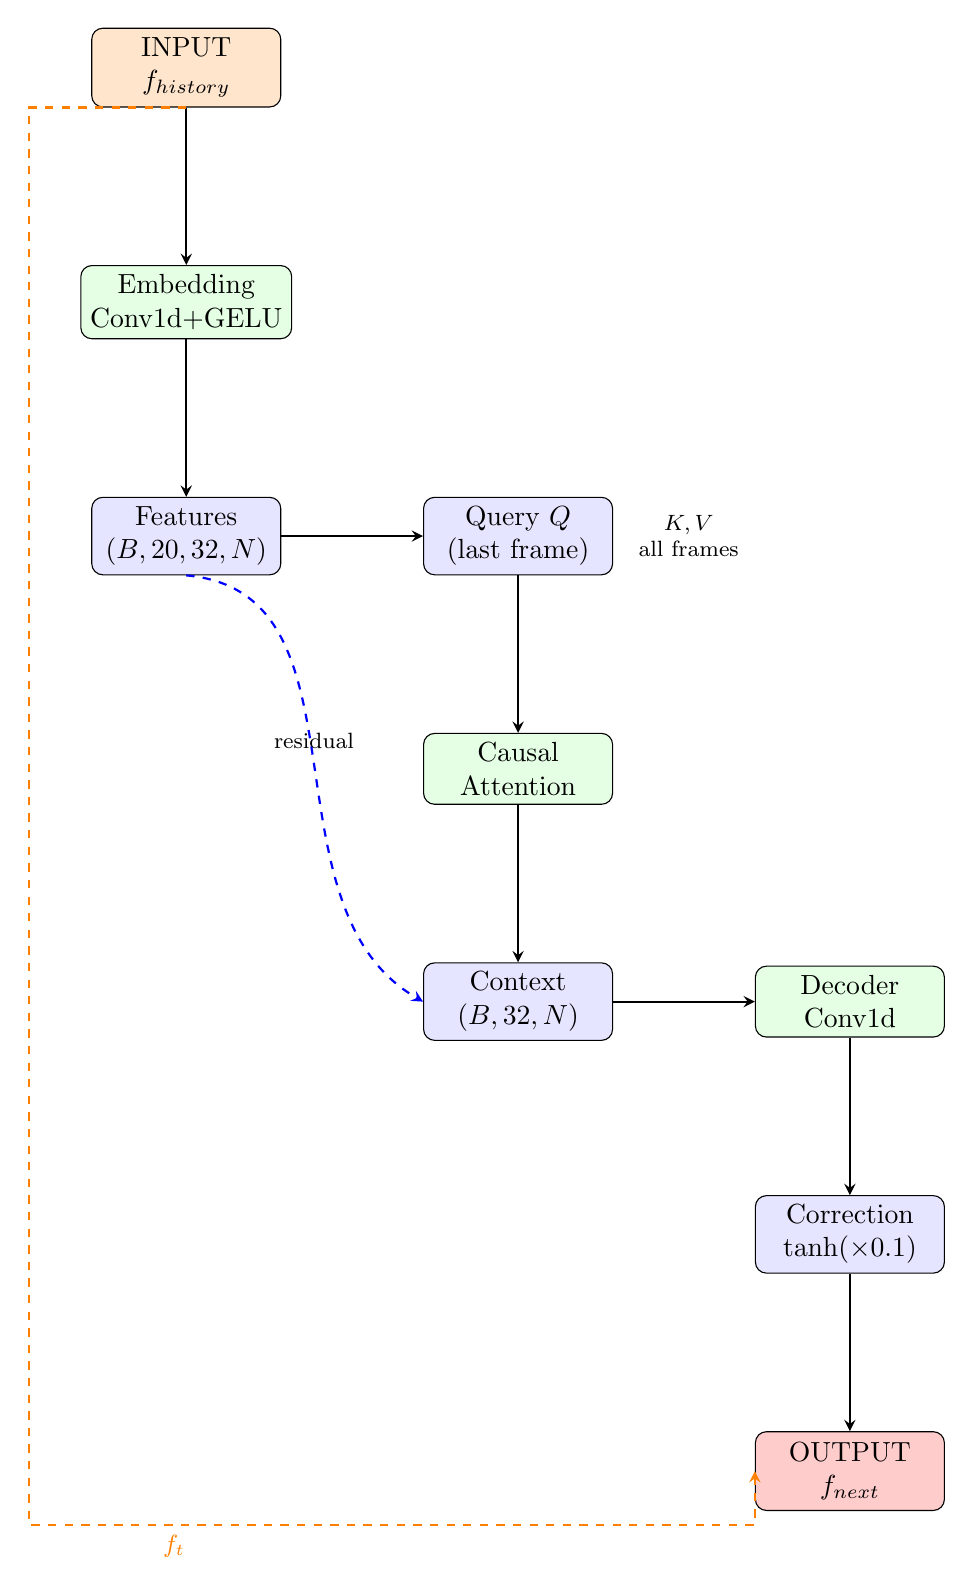
\begin{tikzpicture}[
        box/.style={rectangle, draw, rounded corners, minimum width=2.4cm, minimum height=0.85cm, align=center, fill=blue!10},
        op/.style={rectangle, draw, rounded corners, minimum width=2.4cm, minimum height=0.85cm, align=center, fill=green!10},
        arrow/.style={->, thick, >=stealth},
        input/.style={rectangle, draw, rounded corners, minimum width=2.4cm, minimum height=1.0cm, align=center, fill=orange!20},
        output/.style={rectangle, draw, rounded corners, minimum width=2.4cm, minimum height=1.0cm, align=center, fill=red!20},
        node distance=2.0cm and 1.6cm
    ]
    % Main flow - left column
    \node[input] (input) {INPUT\\$f_{\text{history}}$};
    \node[op, below=of input] (embed) {Embedding\\Conv1d+GELU};
    \node[box, below=of embed] (features) {Features\\$(B,20,32,N)$};

    % Attention column - center-right
    \node[box, right=1.8cm of features] (query) {Query $Q$\\(last frame)};
    \node[op, below=of query] (attn) {Causal\\Attention};
    \node[box, below=of attn] (context) {Context\\$(B,32,N)$};

    % Decoder/output column - right
    \node[op, right=1.8cm of context] (decoder) {Decoder\\Conv1d};
    \node[box, below=of decoder] (corr) {Correction\\$\tanh(\times0.1)$};
    \node[output, below=of corr] (output) {OUTPUT \\$f_{\text{next}}$};

    % CLEAN ARROWS - NO CROSSING
    \draw[arrow] (input) -- (embed);
    \draw[arrow] (embed) -- (features);
    \draw[arrow] (features) -| ([xshift=-0.3cm]query.west) -- (query);
    \draw[arrow] (query) -- (attn);
    \draw[arrow] (attn) -- (context);
    \draw[arrow] (context) -- (decoder);
    \draw[arrow] (decoder) -- (corr);
    \draw[arrow] (corr) -- (output);

    % Residual from features to context (ABOVE)
    \draw[arrow, dashed, blue] (features.south) 
        to[out=-5,in=150] node[above, font=\footnotesize, black]{residual} 
        (context.west);

    % FIXED: LEFT→DOWN→RIGHT path from input to output
    \draw[arrow, dashed, orange, thick] (input.south) 
        |- ++(-2,0)     % LEFT (west)
        |- ++(0,-18)     % DOWN (south) 
        -| (output.west)     % RIGHT to output
        node[below, font=\small, pos=0.1]{$f_t$};


    % KV note
    \node[font=\footnotesize, align=center, right=0.2cm of query, anchor=west] (kv) {$K,V$\\all frames};
    \end{tikzpicture}%
}
\caption{Data flow through the Causal Temporal Attention Network during one prediction step.}
\label{fig:tcn-flow}
\end{figure}

\subsection{Autoregressive Training Procedure}

Training uses \textbf{curriculum learning} with multi-step rollouts ($D=8\to16\to64$):

\begin{enumerate}
    \item Initialize $\text{window} = f_{\text{ground\_truth}}[:, :20, :]$ from ground truth trajectories.
    
    \item For each rollout step $k \in \{0, \dots, D-1\}$ where $D$ is the rollout depth:
    \begin{itemize}
        \item Predict $\hat{f}_{20+k} = \text{TCAN}(\text{window})$.
        \item Compute physics-informed loss:
        \[
        \mathcal{L}
        = \text{MSE}(\hat{f}, f_{\text{ground\_truth}})
        + 0.1 \, \|\nabla_x \hat{f} - \nabla_x f_{\text{ground\_truth}}\|^2
        + 0.05 \, \mathbb{E}\!\left[\max\!\left(0, E(\hat{f}) - E(f_t)\right)\right]
        \]
        where 
        \[
        E(u) = \frac{1}{2} \int u^2 \, dx
        \] enforces energy dissipation.
        \item Update window: $\text{window} \gets [\text{window}[:, 1:, :], \hat{f}]$ (with occasional teacher forcing).
    \end{itemize}
    
    \item Average loss over rollout, backpropagate through unrolled computation graph, apply gradient clipping, and optimize with AdamW + cosine annealing.
\end{enumerate}

\subsection{Training Progress and Results}
Figure~\ref{fig:training-progress} shows TCAN predictions every 20 epochs over 100 total epochs.
% ---------------------------- TRAINING PROGRESS FIGURE ----------------------------
\begin{figure}[h!]
\centering

% Row 1 (2 large subfigures)
\includegraphics[width=0.48\textwidth, height=1.8cm]{images/trajectory_epoch_0_nu0.2.png}\hfill
\includegraphics[width=0.48\textwidth, height=1.8cm]{images/trajectory_epoch_20_nu0.2.png}\hfill

\vspace{0.4cm}

% Row 2 (2 large subfigures)
\includegraphics[width=0.48\textwidth, height=1.8cm]{images/trajectory_epoch_40_nu0.2.png}\hfill
\includegraphics[width=0.48\textwidth, height=1.8cm]{images/trajectory_epoch_60_nu0.2.png}\hfill

\vspace{0.4cm}

% Row 3 (2 large subfigures)
\includegraphics[width=0.48\textwidth, height=1.8cm]{images/trajectory_epoch_80_nu0.2.png}\hfill
\includegraphics[width=0.48\textwidth, height=1.8cm]{images/trajectory_epoch_100_nu0.2.png}

\caption{TCAN training evolution ($\nu=0.2$). Epochs 0$\to$20 (top), 40$\to$60 (middle), 80$\to$100 (bottom).}
\label{fig:training-progress}
\end{figure}


%------------------------------ LOSS CURVE FIGURE ----------------------------

Figure~\ref{fig:loss-curve} displays the composite loss over the evaluation loop, showing steady decrease and saturation after epoch 70, confirming training stability.

\begin{figure}[h!]
\centering
\includegraphics[width=0.6\textwidth]{images/losses_over_epochs.png}
\caption{Composite training loss ($\mathcal{L}$) over evaluation loop across 100 epochs. Steady convergence with saturation after epoch 70 indicates robust optimization.}
\label{fig:loss-curve}
\end{figure}


\subsubsection{Evaluation Metrics}
% ---------- RESULTS + EVALUATION METRICS --------------------
Full-trajectory predictions are assessed with comprehensive metrics (Table~\ref{tab:tcn-metrics}):

\begin{table}[h!]
\centering
\resizebox{1.1\textwidth}{!}{
\begin{tabular}{@{\extracolsep{14pt}}l@{\extracolsep{14pt}}c@{\extracolsep{14pt}}l@{\extracolsep{14pt}}c@{\extracolsep{14pt}}c}
\toprule
\textbf{Metric} & \textbf{Formula} & \textbf{Purpose} & \textbf{Good} & \textbf{Failure} \\
\midrule[1pt]
MSE & $\frac{1}{NP}\sum(u_\text{pred}-u_\text{gt})^2$ & Pixel accuracy & $<10^{-4}$ & $>10^{-3}$ \\
Rel. $L^2$ & $\|u_\text{pred}-u_\text{gt}\|_2/\|u_\text{gt}\|_2$ & Scale-invariant & $<0.05$ & $>0.2$ \\
PSNR & $20\log(\text{range}/\sqrt{\text{MSE}})$ & Image quality & $>30$dB & $<20$dB \\
SSIM & Structural similarity & Texture preservation & $>0.9$ & $<0.7$ \\
Correlation & Pearson $r$/step & Phase alignment & $>0.95$ & $<0.8$ \\
\hline[0.8pt]
Mass Error & $|\int u\,dx-M_0|$ & Conservation & $<0.01$ & $>0.1$ \\
Energy Monotonicity & $E(t+1)\leq E(t)$ & Dissipation & $>0.95$ & $<0.8$ \\
PDE Residual & $\|F(u)\|_2$ & PDE satisfaction & $<0.01$ & $>0.1$ \\
Max Gradient & $\max|\partial_xu|$ & Shock preservation & $\pm10\%$GT & Diverges \\
Gradient Error & $\|\nabla_x(u_\text{pred}-u_\text{gt})\|_2$ & Shock sharpness & $<0.05$ & $>0.2$ \\
\bottomrule[1pt]
\end{tabular}
}
\caption{TCAN evaluation metrics with formulas, purposes, and thresholds.}
\label{tab:model-metrics}
\end{table}